\documentclass[12pt]{report}

\usepackage{cmap}
\usepackage[T1,T2A]{fontenc}
\usepackage[utf8]{inputenc}
\usepackage[english, russian]{babel}
\usepackage{amssymb}
\usepackage{amsmath}
\usepackage{amsthm}
\usepackage{dsfont}
\usepackage{bm}
\usepackage{diagbox}
\usepackage[left=20mm,right=10mm,top=20mm,bottom=20mm,bindingoffset=2mm]{geometry}
\usepackage{indentfirst}
\usepackage[utf8]{inputenc}
\usepackage{float}
\usepackage[hidelinks]{hyperref}
\usepackage{graphicx}
\usepackage{xcolor}
\usepackage{listings}
\usepackage{minted}

\DeclareMathOperator{\N}{\mathbb{N}}
\DeclareMathOperator{\R}{\mathbb{R}}
\DeclareMathOperator{\Z}{\mathbb{Z}}
\DeclareMathOperator{\CC}{\mathbb{C}}
\DeclareMathOperator{\PP}{\mathrm{P}}
\DeclareMathOperator{\Expec}{\mathrm{E}}
\DeclareMathOperator{\Var}{\mathrm{Var}}
\DeclareMathOperator{\Cov}{\mathrm{Cov}}
\DeclareMathOperator{\asConv}{\xrightarrow{a.s.}}
\DeclareMathOperator{\LpConv}{\xrightarrow{Lp}}
\DeclareMathOperator{\pConv}{\xrightarrow{p}}
\DeclareMathOperator{\dConv}{\xrightarrow{d}}

\hypersetup{
	colorlinks=true,
	linkcolor=blue,
	citecolor=blue,
	urlcolor=blue
}

\lstset{language=Python, extendedchars=\true}

\lstdefinestyle{pythonstyle}{
	language=Python,
	backgroundcolor=\color{lightgray},
	commentstyle=\color{green},
	keywordstyle=\color{blue},
	stringstyle=\color{red},
	basicstyle=\ttfamily,
	frame=single,
	breaklines=true
}

\begin{document}
	
	\begin{titlepage}
		\begin{center}
			\large{Федеральное государственное автономное образовательное учреждение высшего образования <<Национальный исследовательский университет ИТМО>>}
		\end{center}
		
		\vspace{15em}
		
		\begin{center}
			\huge{\textbf{Лабораторная работа №1}} \\
			\large{По дисциплине <<Системы искусственного интеллекта>>} \\
		\end{center}
		
		\vspace{5em}
		
		\begin{flushright}
			\textit{\large{Выполнил:}} \\
			\large{Студент группы P3306} \\
			\large{Михайлов Дмитрий} \\
			\large{Андреевич} \\
			\textit{\large{Преподаватель:}} \\
			\large{Кугаевских Александр} \\
			\large{Владимирович}
		\end{flushright}
		
		\vspace{2cm}
		
		\begin{figure}[h]
			\centering
			
\includegraphics[width=0.5\linewidth]{image.png}
		\end{figure}
		
		\begin{center}
			Санкт-Петербург \\
			2025 год
		\end{center}
	\end{titlepage}
	
	\tableofcontents
	\newpage
	
	\addcontentsline{toc}{section}{Цель работы}
	\section*{Цель работы}
	Создание базы знаний в среде Prolog, используя своё генеалогическое древо.
	
	\begin{flushleft}
		Предметная область - Ваше семейное дерево
		
		\begin{itemize}
			\item Создать не менее 30 объектов - членов вашей семьи.
			\item Факты, отражающие состояние - события, регистрируемые органами ЗАГС (рождение, смерть, заключение брака, расторжение брака).
			\item Создать не менее 30 правил, определяющих на основании событий состояния членов семьи и отношения между ними.
			\item Правила должны учитывать темпоральность состояний с точностью до года.
		\end{itemize}
		
	\end{flushleft}
	
	\begin{flushleft}
		Содержание отчёта:
		
		\begin{itemize}
			\item Семейное дерево (можно хоть от руки). 
			\item Список фактов с описанием аргументов. 
			\item Список правил с комментариями. 
			\item Не менее 10 скриншотов с результатами выполнения запросов. Запросы могут быть примерно такими: На ком был ХХХ женат в 1997 году? Запросы НЕ на естественном языке. На Прологе. 
		\end{itemize}
		
	\end{flushleft}
	
	\addcontentsline{toc}{section}{Ход работы}
	\section*{Ход работы}
	
	\begin{figure}[htbp]
		\centering
		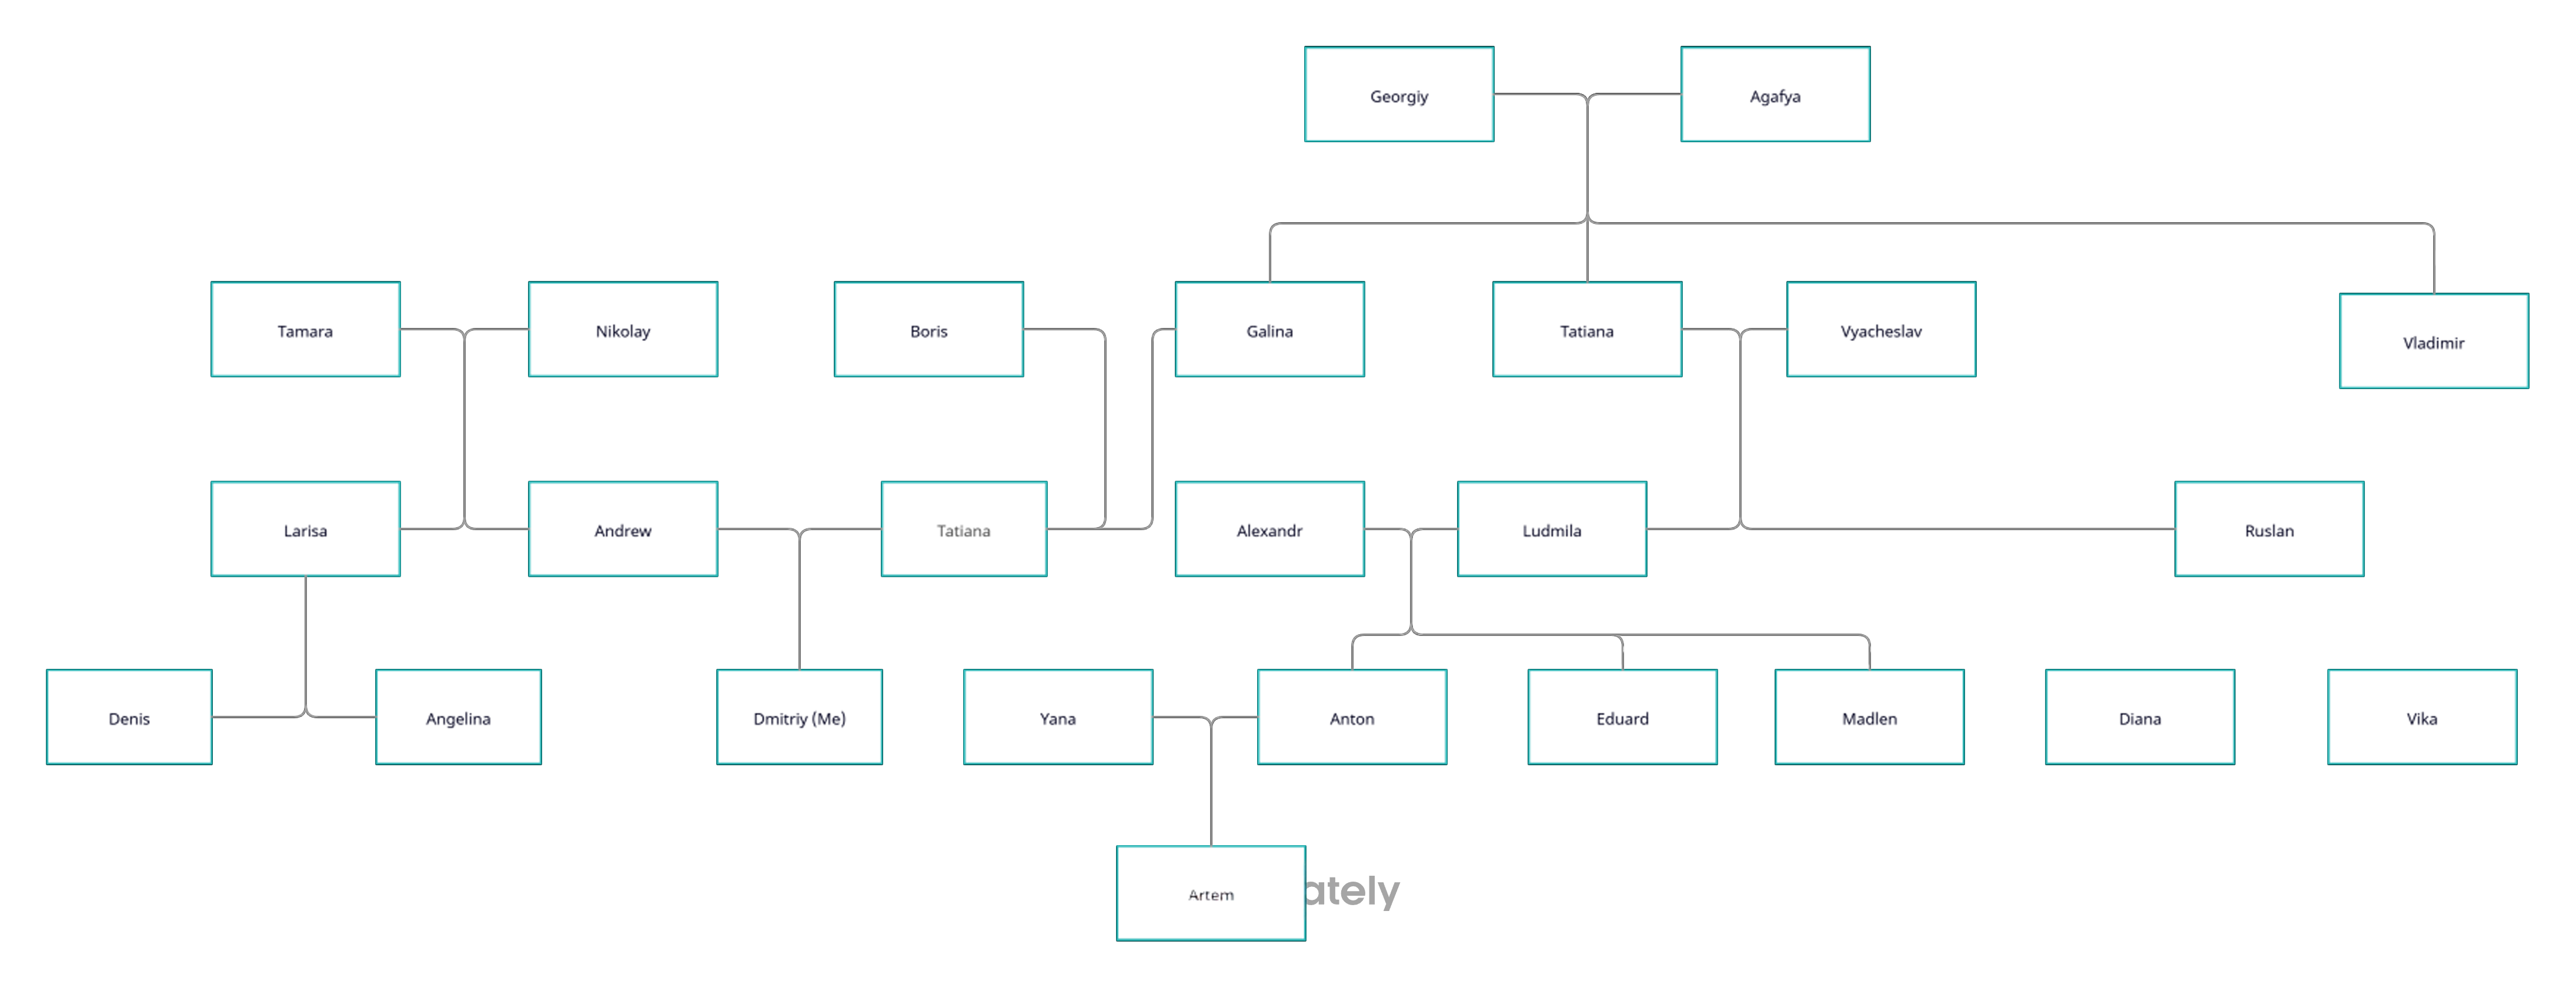
\includegraphics[width=0.6\textwidth]{derevo.png}
		\caption{Генеологическое дерево.}
		\label{fig:genealog_tree}
	\end{figure}
	\newpage
	
	\addcontentsline{toc}{section}{Листинг программы}
	\section*{Листинг программы}
	\href{https://github.com/mysticslippers/artificial_intelligence_systems_archive/blob/main/Lab1_ais/code/src.pl}{Ссылка на репозиторий с кодом.}
	
	
	
	\addcontentsline{toc}{section}{Результат выполнения программы}
	\section*{Результат выполнения программы}
	
	\begin{figure}[h]
		\centering
		\includegraphics[width=0.6\linewidth]{screenshot.jpg}
	\end{figure}
	
	\addcontentsline{toc}{section}{Вывод}
	\section*{Вывод}
	В результате выполнения данной лабораторной работы я познакомился с языком программирования Prolog, который основан не на алгоритме, а на логике предикатов, с помощью которых можно описывать логических процессов и выстраивать взаимосвязи, а также применила полученные знания на практике и построила генеологическое дерево с помощью Prolog.
\end{document}
